\documentclass[12pt, a4paper]{report}
\usepackage{graphicx, array, amsthm, amssymb, amsmath, algorithm, algpseudocode, float, xcolor, thmtools, thmbox, exercise}
\usepackage[english]{babel}

\makeatletter
\renewcommand\thmbox@headstyle[2]{\bfseries #1}
\makeatother
\newtheorem[style=M,bodystyle=\normalfont]{theorem}{Theorem}
\newtheorem[style=M,bodystyle=\normalfont]{corollary}{Corollary}
\newtheorem[style=M,bodystyle=\normalfont]{lemma}{Lemma}
\newtheorem[style=M,bodystyle=\normalfont]{definition}{Definition}


\title{Formal Languages And Compilers \\ \textit{Exercises}}
\author{Christian Rossi}
\date{Academic Year 2023-2024}

\begin{document}

\maketitle

\newpage

\begin{abstract}
    The lectures are about those topics: 
    \begin{itemize}
        \item Definition of language, theory of formal languages, language operations, regular expressions, regular languages, finite deterministic and non-deterministic automata, 
            BMC and Berry-Sethi algorithms, properties of the families of regular languages, nested lists and regular languages.
        \item Context-free grammars, context-free languages, syntax trees, grammar ambiguity, grammars of regular languages, properties of the families of context-free languages, 
            main syntactic structures and limitations of the context-free languages.
        \item Analysis and recognition (parsing) of phrases, parsing algorithms and automata, push down automata, deterministic languages, bottom-up and recursive top-down syntactic 
            analysis, complexity of recognition.
        \item Syntax-driven translation, direct and inverse translation, syntactic translation schemata, transducer automata, and syntactic analysis and translation. Definition of 
            semantics and semantic properties. Static flow analysis of programs. Semantic translation driven by syntax, semantic functions and attribute grammars, one-pass and 
            multiple-pass computation of the attributes.
    \end{itemize}
    The laboratory sessions are about those topics: 
    \begin{itemize}
        \item Modellization of the lexicon and the syntax of a simple programming language (C-like).
        \item Design of a compiler for translation into an intermediate executable machine language (for a register-based processor).
        \item Use of the automated programming tools Flex and Bison for the construction of syntax-driven lexical and syntactic analyzers and translators.
    \end{itemize}
\end{abstract}

\newpage

\tableofcontents

\newpage

\chapter{Exercise session I}

    \section{Regular expression's equality}
        Given two regular expression: 
        \[R_1=((2b)^{*}c)^* \:\:\:\:\:\:\:\:\:\:\:\: R_2=(c^*(2b)^{*})^*\]
        Check if they are equal. If they are not give a counterexample. 
    \subsection*{Solution}
        It is possible to see that $R_1$ and $R_2$ are not equivalent because the character $c$ is in a different position and can be found multiple times in $R_2$, while in $R_1$ is 
        found exactly one time. An example can be $ab$. This string is included in the second language, but not in the first one. 

    \newpage 

    \section{Regular expression's ambiguity}
        Given the regular expression: 
        \[R_1=(a|\varepsilon)^{+}(ba|bab)^{*}\]
        check if it is ambiguous. 
    \subsection*{Solution}
        First, we enumerate all the characters in the regular expression, obtaining: 
        \[R_1=(a_1|\varepsilon)^{+}(b_2a_3|b_4a_5b_6)^{*}\]
        and now we try to come up with an ambiguous string to prove that the regular expression is ambiguous. 
        A regular expression is considered ambiguous if there is a string which can be matched by more than one way from the regular expression. 
        For instance, we can have the string $a_1$ can be generated multiple times selecting the $\varepsilon \: n - 1$ times. This proves that the regular expression is ambiguous. 

    \newpage

    \section{Operations on languages}
        Given two regular expressions: 
        \[R_1=a((b|bb)a)^{+} \:\:\:\:\:\:\:\:\:\:\:\: R_2=(ab)^{*}ba\]
        Define the quotient language $L=R_1-R_2$. 
        \begin{enumerate}
            \item Write the three shortest strings of the language $L$.
            \item Write a regular expression that defines the language. 
        \end{enumerate}
    \subsection*{Solution}
        First, we enumerate all the characters in the regular expressions, obtaining: 
        \[R_1=a_1((b_2|b_3b_4)a_5)^{+}\]
        \[R_2=(a_1b_2)^{*}b_3a_4\]
        The $a_1$ is surely a prefix for every string in the language, and all the strings have $a_5$ as a suffix. The shortest strings of this language are: $aba$, $ababa$ and $abababa$. 
        
        For the second regular expression we have that every string generated starts with $ab$ and have a single $ba$ as a suffix. The shortest strings of this language are: $ba$, $abba$ and $abababa$. 
        
        We can see that all the strings that have the suffix $aba$ or have at least two $bb$ are certainly in $L$. 

        \begin{enumerate}
            \item Now, we can see that the three shortest strings are: $aba$, $ababa$, and $abbaba$. 
            \item The regular expression is: 
                \[L=\{(a(b|bb))^{*}aba\} \cup \{(a(b|bb))^{*}abba(a(b|bb))^{+}abba\}\]
        \end{enumerate}    
    
\newpage

\chapter{Exercise session II}
    \section{Regular expressions and FSA}
        Consider the regular expression $R$ below, over the three-letter alphabet $\Sigma=\{a,b,c\}$ 
        \[R=a\left( b|c^{+}a \right)^{*}\]
        Answer the following questions:
        \begin{enumerate}
            \item Write all the strings $x$ of the language of $R$ that have a length less than or equal to four, i.e., $x \in L(R)$ with $|x| \leq 4$, in lexicographic order 
                (with $a < b < c$).
            \item By means of the Berry-Sethi method, find a deterministic automaton $A$ equivalent to the regular expression $R$. 
            \item Is the deterministic automaton $A$ found before minimal? Justify your answer.
            \item By means of the Brzozowski method (node elimination), starting from the automaton $A$ found before, obtain a regular expression $R^{'}$ equivalent to $A$.
            \item Is the language $L(R)$ locally testable? Formally prove your answer.
        \end{enumerate}
    \subsection*{Solution}
    \begin{enumerate}
        \item The possible strings are: $a$, $ab$, $abb$, $aca$, $abba$, $abca$, $acab$, $acca$. 
        \item First, we enumerate the symbols $R_{\#}=a_1\left( b_2|c^{+}_{3}a_4 \right)^{*}\dashv$. We construct the following support table: 
            \begin{table}[H]
                \centering
                \begin{tabular}{cc}
                Initials                       & $a_1$             \\ \hline
                \multicolumn{1}{c|}{Terminals} & Followers         \\
                \multicolumn{1}{c|}{$a_1$}     & $b_2c_3\dashv$ \\
                \multicolumn{1}{c|}{$b_2$}     & $b_2c_3\dashv$  \\
                \multicolumn{1}{c|}{$c_3$}     & $c_3a_4$         \\
                \multicolumn{1}{c|}{$a_4$}     & $b_2c_3\dashv$ 
                \end{tabular}
            \end{table}
            We start wit the initial, and we have: 
            \begin{figure}[H]
                \centering
                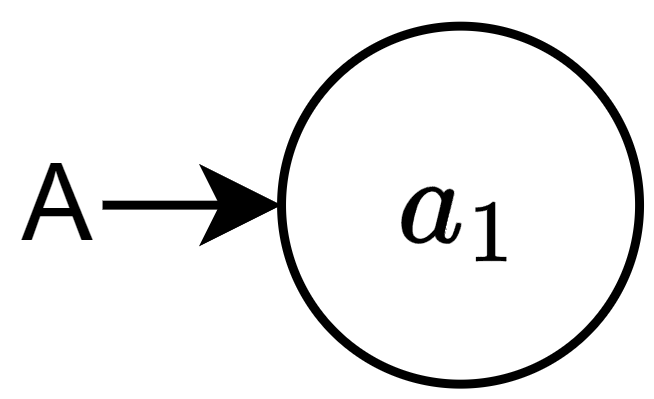
\includegraphics[width=0.2\linewidth]{images/FSA1.png}
            \end{figure}
            Now we create the state reachable from $a_1$, and we obtain: 
            \begin{figure}[H]
                \centering
                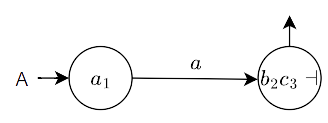
\includegraphics[width=0.4\linewidth]{images/FSA2.png}
            \end{figure}
            After doing this steps for all the states we obtain the following automaton: 
            \begin{figure}[H]
                \centering
                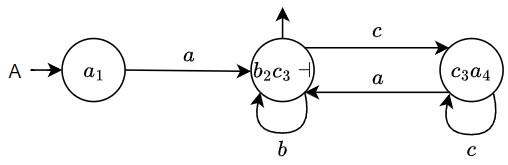
\includegraphics[width=0.5\linewidth]{images/FSA3.png}
            \end{figure}
        \item We can reduce an automaton if we can reduce the number of states. We have to use some criterions to do the check on automaton $A$. To simplify the automaton we start by renaming the states: 
            \begin{figure}[H]
                \centering
                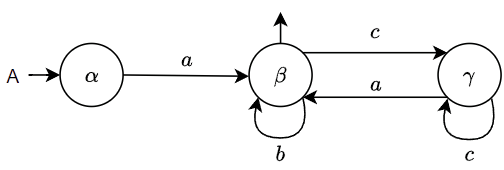
\includegraphics[width=0.5\linewidth]{images/FSA4.png}
            \end{figure}
            We can see that $\alpha$ cannot be merged with $\beta$ because one is not final and the other one is final. 
            Same reasoning holds for $\beta$ and $\gamma$. States $\alpha$ and $\gamma$ cannot be merged because they have different transitions. 
            So, the three states are distinguishable, and the automaton is the minimal. 
        \item We start by creating a virtual initial node and final node connected to the automata: 
            \begin{figure}[H]
                \centering
                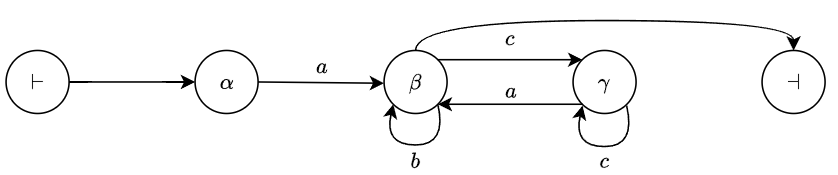
\includegraphics[width=0.75\linewidth]{images/FSA5.png}
            \end{figure}
            Now we can remove the states one by one until we reach the final state directly from the initial one. 
            So, we remove $\gamma$ with the loop $c^{+}a$. We have two cycles on $\beta$ that can be substituted by the expression
            $(b|c^{+}a)^{*}$. We have only $\alpha$ that can be easily removed, and we finally have that: 
            \[R^{'}=a(b|c^{+}a)^{*}\]
        \item We have the following sets: 
            \begin{itemize}
                \item Initials: $\{a\}$
                \item Finals: $\{a,b\}$
                \item Digrams: $\{aa,ac,bb,bc,ca,cc\}$
            \end{itemize}
            Using these sets we can build a particular automaton $A^{'}$, that have the initial set connected to the set of initials, the final states are the ones in the finals set, and the transitions are the
            one belonging to the digrams set. 
            \begin{figure}[H]
                \centering
                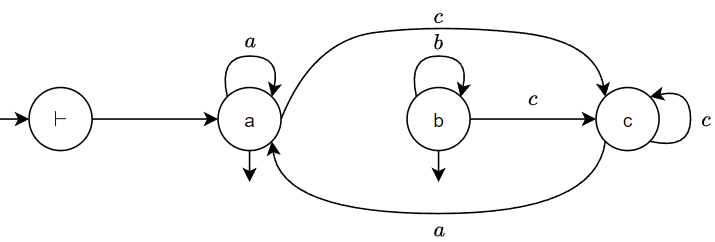
\includegraphics[width=0.75\linewidth]{images/FSA6.png}
            \end{figure}
            The automaton is local if it recognizes the initial language and if the edge reached by an arc has the same name of the transition. In this case we constructed the nodes such that the second property is 
            satisfied, so we simply need to check the first property. We can not that the states $a$ and $b$ are not distinguishable, so we can reduce the automaton to the $A$ one. So, the language is locally testable. 
    \end{enumerate}

    \newpage

    \section{Regular expressions and FSA}
        Take a two-letter alphabet $\Sigma=\{a,b\}$.  Consider the nondeterministic automaton $A$ over $\Sigma$ below, which has spontaneous transitions ($\varepsilon$-transitions): 
        \begin{figure}[H]
            \centering
            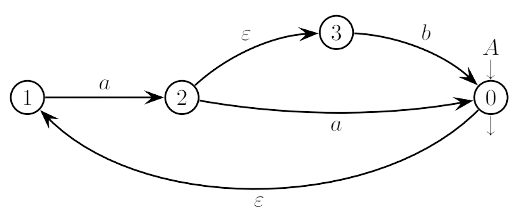
\includegraphics[width=0.5\linewidth]{images/FSA1a.png}
        \end{figure}
        And consider also the regular expression $R$ over $\Sigma$ below:
        \[R=\left( aa|ab|ba \right)^{*}\]
        Answer the following questions:
        \begin{enumerate}
            \item Find all the valid strings of language $L(A)$ that have a length less or equal than four. Do the same for language $L(R)$, too.
            \item By using the back propagation method, eliminate the spontaneous transitions of automaton $A$ and obtain an equivalent deterministic automaton $A_1$ without spontaneous transitions. 
                Clean and minimize automaton $A_1$, if necessary. Test automaton $A_1$ with the valid short strings found at point one for automaton $A$. 
            \item By using the Berry-Sethi method, obtain a deterministic automaton $A_2$ equivalent to the regular expression $R$. Minimize automaton $A_2$, if necessary. Test automaton $A_2$ with the valid short 
                strings found at point one for expression $R$.
            \item Say if language $L(R)$ is local or not, and shortly justify your answer.
            \item By using a systematic method of your choice, obtain a deterministic automaton $A_3$ for the difference language $L_D=L(R)-L(A)$, i.e., $L(R) \cap \overline{L(A)}$, which contains the strings generated 
                by $R$ that are not recognized by $A$. Then test automaton $A_3$: by examining (only) the strings of length 4 found at point one, find in alphabetical order the first two strings $x$ and $y$ such that
                $x \in L_D$ and $y \notin L_D$, and show that $x \in L(A_3)$ and $y \notin L(A_3)$.
        \end{enumerate}
    \subsection*{Solution}
        \begin{enumerate}
            \item The strings of the language $L(A)$ are $\varepsilon$, $aa$, $ab$, $aaaa$, $aaab$, $abaa$, and $abab$. 
                The strings of the language $L(R)$ are: $\varepsilon$, $aa$, $ab$, $ba$, $aaaa$, $aaab$, $aaba$, $abaa$, $abab$, $abba$, $baaa$, $baab$, and $baba$. 
            \item The idea of the back propagation method is to start from the arriving state of an $\varepsilon$ transition, eliminate the spontaneous transition and back propagate the transition exiting from the state.
                In this case we obtain the following automaton: 
                \begin{figure}[H]
                    \centering
                    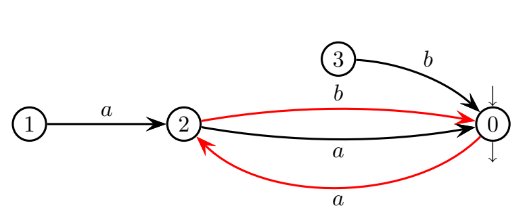
\includegraphics[width=0.5\linewidth]{images/FSA2a.png}
                \end{figure}
                After that we can remove the useless states and rename the remaining ones. 
                \begin{figure}[H]
                    \centering
                    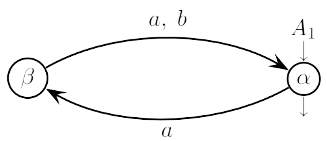
\includegraphics[width=0.5\linewidth]{images/FSA3a.png}
                \end{figure}
                The states are un-distinguishable, so the automaton is the minimal one, and it is the same as the initial one. 
            \item First, we enumerate the symbols $R_{\#}=\left( a_1a_2|a_3b_4|b_5a_6 \right)^{*}\dashv$. We construct the following support table: 
                \begin{table}[H]
                    \centering
                    \begin{tabular}{cc}
                    Initials                       & $a_1a_3a_5\dashv$              \\ \hline
                    \multicolumn{1}{c|}{Terminals} & Followers                      \\
                    \multicolumn{1}{c|}{$a_1$}     & $a_2$                          \\
                    \multicolumn{1}{c|}{$a_2$}     & $a_1a_3a_5\dashv$              \\
                    \multicolumn{1}{c|}{$a_3$}     & $b_4$                          \\
                    \multicolumn{1}{c|}{$b_4$}     & $a_1a_3a_5\dashv$              \\
                    \multicolumn{1}{c|}{$b_5$}     & $a_6$                          \\
                    \multicolumn{1}{c|}{$a_6$}     & $a_1a_3a_5\dashv$ 
                    \end{tabular}
                \end{table}
                From which we construct the following automaton: 
                \begin{figure}[H]
                    \centering
                    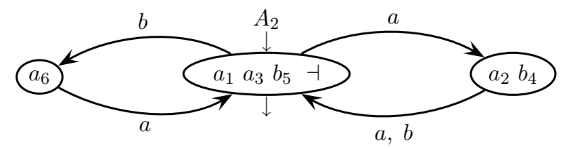
\includegraphics[width=0.75\linewidth]{images/FSA4a.png}
                \end{figure}
                That is already minimal. 
            \item The language is not local. The minimal automaton of a local language is necessarily local. Automaton $A_2$ is minimal, but it is not local. Thus, language $L(R)$ is not local.
            \item The language $L_D=L(R)-L(A)=L(R) \cup \overline{L(A)}$. We need to find the complement of the automaton $A$, by switching final and non-final states with the complement, and by adding 
                an error state $\eta$. In this case we obtain:
                \begin{figure}[H]
                    \centering
                    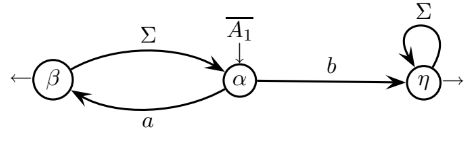
\includegraphics[width=0.5\linewidth]{images/FSA5a.png}
                \end{figure}
                We rewrite the automaton $A_2$
                \begin{figure}[H]
                    \centering
                    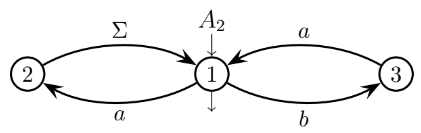
\includegraphics[width=0.5\linewidth]{images/FSA6a.png}
                \end{figure}
                We can write all the states and then try to connect with both transitions, and so we obtain: 
                \begin{figure}[H]
                    \centering
                    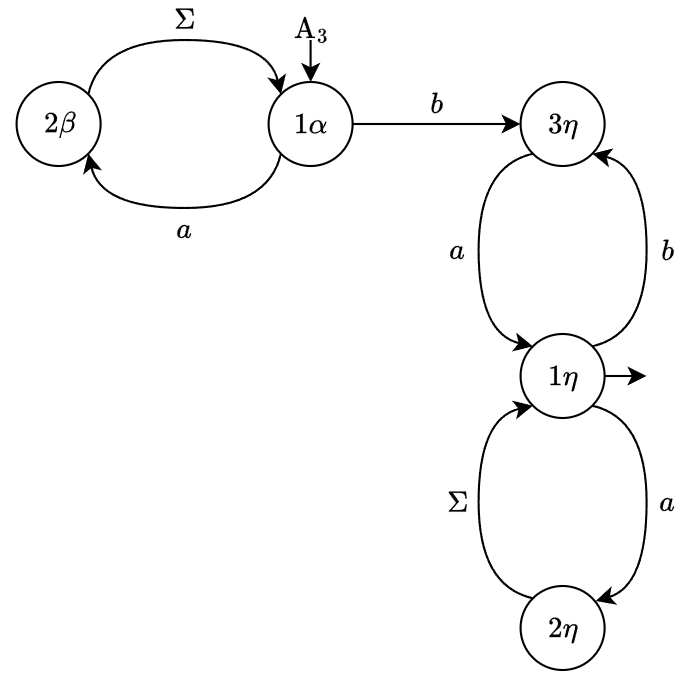
\includegraphics[width=0.5\linewidth]{images/FSA7a.png}
                \end{figure}
                Automaton $A_3$ has five states only. It is deterministic, as both factor automata are so. It is clean, though it might not be minimal. Here is the test of automaton $A_3$. From question one, 
                alphabetically list the length-4 strings of language $L(R)$ and, similarly, those of language $L(A)$. Then in the first list pick the first string $x$ that is not in the second list, and the first 
                string $y$ that is also in the second list. Result: $x=a a b$ a and $y=a a a a$. We soon see that $x \in L(A_3)$ and $y \notin L(A_3)$. Thus, automaton $A_3$ passes this test successfully.
        \end{enumerate}

\newpage 

\chapter{Exercise session III}
    \section{Free Grammars and PDA}
        Given the alphabet $\Sigma=\{a,b\}$ and the languages $L_1=\{ww^R|w \in \Sigma^{+}\}$ and $L_2=(b^{*}a^{*}b^{*})$.
        \begin{enumerate}
            \item Define a grammar for $L_1$ and $L_2$. 
            \item Find the intersection of the two grammars. 
            \item Find the intersection $L_1 \cap (b^{*}a^{*}b^{*}a^{*})$
        \end{enumerate}
    \subsection*{Solution}
    \begin{enumerate}
        \item The grammar for the first language is the following: 
            \[\begin{cases}
                S_1 \rightarrow aS_1a           \\
                S_1 \rightarrow bS_1b           \\
                S_1 \rightarrow \varepsilon
            \end{cases}\]
            The grammar for the second language is: 
            \[\begin{cases}
                S_1 \rightarrow bS_1|X          \\
                X \rightarrow aX|Y              \\
                Y \rightarrow bY|\varepsilon
            \end{cases}\]
        \item The intersection between the two grammars is: 
            \[L=(b^na^mb^n)\]
            where $n \geq 0$, and $m \geq 0$ an even number. The corresponding grammar is the following: 
            \[\begin{cases}
                S_1 \rightarrow bS_1b | X \\
                X \rightarrow aXa | \varepsilon
            \end{cases}\]
        \item The intersection of the languages is: 
            \[\begin{cases}
                S_1 \rightarrow X | U               \\
                X \rightarrow bXb | Y               \\
                Y \rightarrow aYa | \varepsilon     \\
                U \rightarrow aUa   
            \end{cases}\]
    \end{enumerate}

    \newpage
    \section{Syntax analysis and parsing}
    Consider the grammar $G$ below, represented as a machine net, over a three-letter terminal alphabet $\Sigma=\{a,b,c\}$ and a one-letter non-terminal alphabet (axiom $S$):
    \begin{figure}[H]
        \centering
        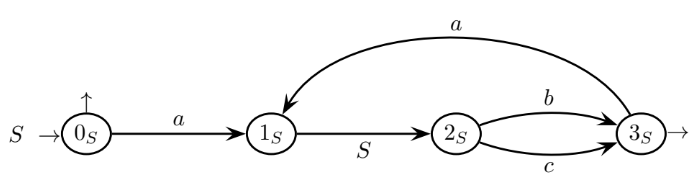
\includegraphics[width=0.5\linewidth]{images/mnet.png}
    \end{figure}
    Answer the following questions:
    \begin{enumerate}
        \item Draw the complete pilot of grammar $G$ and show that grammar $G$ is ELR(1).
        \item Write all the guide sets of the machine net of grammar $G$ (on the call arcs and exit arrows) and show that grammar $G$ is ELL(1).
        \item Write a simulation of the bottom-up analysis of the valid string below:
            \[a a b a c b \in L(G)\]
            Show at least the stack contents, the parsing actions and the resulting syntax tree.
        \item Write the recursive descent procedure for non-terminal $S$, based on the ELL method.
    \end{enumerate}
    \subsection*{Solution}
    \begin{enumerate}
        \item The initial state is the same as the one in the given machine. The final state have a circle surrounding the name. The machine is the following: 
            \begin{figure}[H]
                \centering
                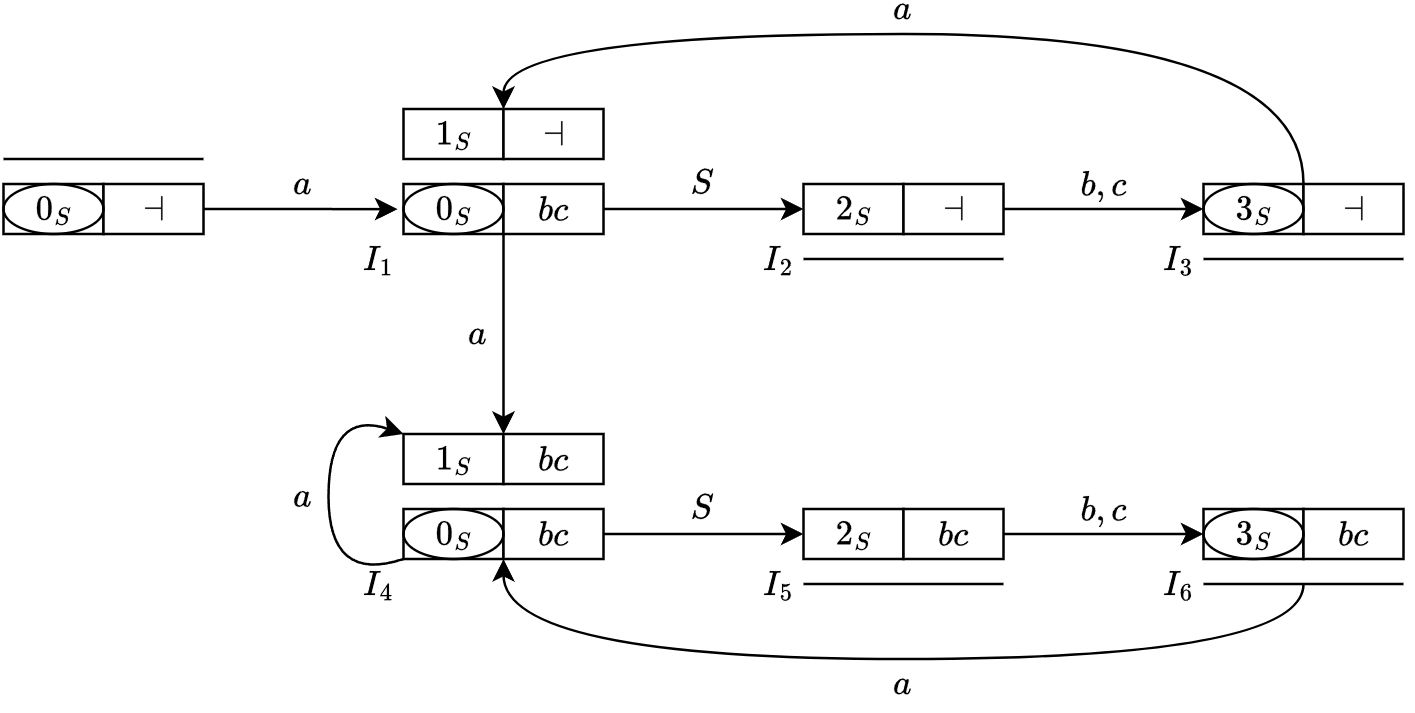
\includegraphics[width=0.6\linewidth]{images/pilot.png}
            \end{figure} 
    \end{enumerate}




\newpage 

\chapter{Exercise session IV}


\newpage 

\chapter{Exercise session V}



\end{document}